
\documentclass[a4paper,12pt]{scrbook}
\usepackage{amsmath,amssymb,amsthm}
\usepackage{fancyvrb}
\usepackage{parskip}
\usepackage{lastpage}
\usepackage{verbatim,boxedminipage,enumitem}
\usepackage{ifthen}
\usepackage{color,graphicx}
\usepackage{pgf}
\usepackage{longtable}
\usepackage{upquote}
%\usepackage[all]{xy}
\usepackage{tobiShell}
\usepackage{tikz}
\usetikzlibrary{automata}
\usetikzlibrary{arrows}
\usepackage{pgf,pgfarrows,pgfnodes}
\usepackage{pgfplots}
\usepackage{circuitikz}
\usetikzlibrary{circuits}
\usetikzlibrary{circuits.logic.US}
\usepackage{mymath}
\usepackage{python}
%------------------------------------------------------------------
% Verbatim for console window - single line frame, no line numbers
%------------------------------------------------------------------
\DefineVerbatimEnvironment%
 {console}{Verbatim}
 {frame=single}

%--------------------------------------------------------
% Remove the vertical spacing before and after Verbatim.
%--------------------------------------------------------
\usepackage{atbeginend}
\BeforeBegin{console}{\mbox{}\\ \begin{minipage}{\textwidth}\vspace{3pt}}
\AfterEnd{console}{\vspace{4pt} \end{minipage} \\ }

\begin{document}
\thispagestyle{empty}

\begin{center}
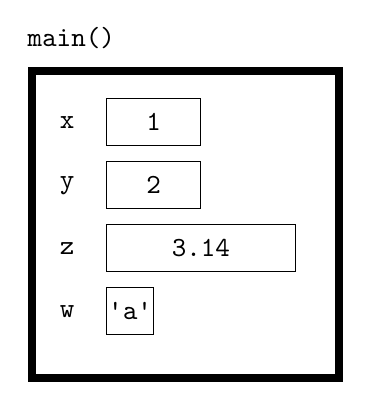
\begin{tikzpicture}

\draw (1.0, -1.0)
  node[draw, line width=0.1cm, , color=black,
       rounded corners=0.0cm, inner sep=0.0cm] {

\begin{minipage}[t][3.9cm]{3.9cm}
\mbox{}

\end{minipage}

};
\draw (1.0, 1.25) node[color=black,
 inner sep=0.0cm] {
 
\begin{minipage}[t][0.5cm]{4.0cm}
{\verb!main()!}
\end{minipage}

};\draw[, font=\ttfamily] (-0.5, 0.3) node {x};

\draw (0.6, 0.3)
  node[draw, , , color=black,
       rounded corners=0.0cm, inner sep=0.0cm] {

\begin{minipage}[t][0.6cm]{1.2cm}
\mbox{}

\end{minipage}

};\draw[, font=\ttfamily] (0.6, 0.3) node {1};
\draw[, font=\ttfamily] (-0.5, -0.5) node {y};

\draw (0.6, -0.5)
  node[draw, , , color=black,
       rounded corners=0.0cm, inner sep=0.0cm] {

\begin{minipage}[t][0.6cm]{1.2cm}
\mbox{}

\end{minipage}

};\draw[, font=\ttfamily] (0.6, -0.5) node {2};
\draw[, font=\ttfamily] (-0.5, -1.3) node {z};

\draw (1.2, -1.3)
  node[draw, , , color=black,
       rounded corners=0.0cm, inner sep=0.0cm] {

\begin{minipage}[t][0.6cm]{2.4cm}
\mbox{}

\end{minipage}

};\draw[, font=\ttfamily] (1.2, -1.3) node {3.14};
\draw[, font=\ttfamily] (-0.5, -2.1) node {w};

\draw (0.3, -2.1)
  node[draw, , , color=black,
       rounded corners=0.0cm, inner sep=0.0cm] {

\begin{minipage}[t][0.6cm]{0.6cm}
\mbox{}

\end{minipage}

};\draw[, font=\ttfamily] (0.3, -2.1) node {{\verb!'a'!}};
\end{tikzpicture}

\end{center}

\end{document}
